% Options for packages loaded elsewhere
\PassOptionsToPackage{unicode}{hyperref}
\PassOptionsToPackage{hyphens}{url}
%
\documentclass[
]{article}
\usepackage{amsmath,amssymb}
\usepackage{iftex}
\ifPDFTeX
  \usepackage[T1]{fontenc}
  \usepackage[utf8]{inputenc}
  \usepackage{textcomp} % provide euro and other symbols
\else % if luatex or xetex
  \usepackage{unicode-math} % this also loads fontspec
  \defaultfontfeatures{Scale=MatchLowercase}
  \defaultfontfeatures[\rmfamily]{Ligatures=TeX,Scale=1}
\fi
\usepackage{lmodern}
\ifPDFTeX\else
  % xetex/luatex font selection
\fi
% Use upquote if available, for straight quotes in verbatim environments
\IfFileExists{upquote.sty}{\usepackage{upquote}}{}
\IfFileExists{microtype.sty}{% use microtype if available
  \usepackage[]{microtype}
  \UseMicrotypeSet[protrusion]{basicmath} % disable protrusion for tt fonts
}{}
\makeatletter
\@ifundefined{KOMAClassName}{% if non-KOMA class
  \IfFileExists{parskip.sty}{%
    \usepackage{parskip}
  }{% else
    \setlength{\parindent}{0pt}
    \setlength{\parskip}{6pt plus 2pt minus 1pt}}
}{% if KOMA class
  \KOMAoptions{parskip=half}}
\makeatother
\usepackage{xcolor}
\usepackage{longtable,booktabs,array}
\usepackage{calc} % for calculating minipage widths
% Correct order of tables after \paragraph or \subparagraph
\usepackage{etoolbox}
\makeatletter
\patchcmd\longtable{\par}{\if@noskipsec\mbox{}\fi\par}{}{}
\makeatother
% Allow footnotes in longtable head/foot
\IfFileExists{footnotehyper.sty}{\usepackage{footnotehyper}}{\usepackage{footnote}}
\makesavenoteenv{longtable}
\usepackage{graphicx}
\makeatletter
\def\maxwidth{\ifdim\Gin@nat@width>\linewidth\linewidth\else\Gin@nat@width\fi}
\def\maxheight{\ifdim\Gin@nat@height>\textheight\textheight\else\Gin@nat@height\fi}
\makeatother
% Scale images if necessary, so that they will not overflow the page
% margins by default, and it is still possible to overwrite the defaults
% using explicit options in \includegraphics[width, height, ...]{}
\setkeys{Gin}{width=\maxwidth,height=\maxheight,keepaspectratio}
% Set default figure placement to htbp
\makeatletter
\def\fps@figure{htbp}
\makeatother
\ifLuaTeX
  \usepackage{luacolor}
  \usepackage[soul]{lua-ul}
\else
  \usepackage{soul}
\fi
\setlength{\emergencystretch}{3em} % prevent overfull lines
\providecommand{\tightlist}{%
  \setlength{\itemsep}{0pt}\setlength{\parskip}{0pt}}
\setcounter{secnumdepth}{-\maxdimen} % remove section numbering
\ifLuaTeX
  \usepackage{selnolig}  % disable illegal ligatures
\fi
\usepackage{bookmark}
\IfFileExists{xurl.sty}{\usepackage{xurl}}{} % add URL line breaks if available
\urlstyle{same}
\hypersetup{
  pdftitle={CS370 Multiagent Learning and Computational Game Solving Notes and Planning},
  hidelinks,
  pdfcreator={LaTeX via pandoc}}

\title{CS370 Multiagent Learning and Computational Game Solving Notes
and Planning}
\author{}
\date{}

\begin{document}
\maketitle

\textbf{\ul{CS370}}

\textbf{\ul{Multiagent Learning \& Computational Game Solving, Notes \&
Planning}}

\textbf{\ul{Deliverables:}}

\begin{itemize}
\item
  Assignment 1 (Applied Focus)

  \begin{itemize}
  \item
    Due Date: End of February
  \item
    Length: Minimum 1000 words
  \item
    Requirements:

    \begin{itemize}
    \item
      Paper Selection: Choose a central applied paper within the fields
      of multiagent learning or computational game solving.
    \item
      Summary Contents:

      \begin{itemize}
      \item
        Key Findings: Summarize the main results and conclusions of the
        paper.
      \item
        Techniques Used: Describe the methodologies and approaches
        employed in the research.
      \item
        Future Work Directions: Identify and discuss potential avenues
        for future research suggested by the paper.
      \end{itemize}
    \end{itemize}
  \end{itemize}
\item
  Assignment 2 (Theoretical Focus)

  \begin{itemize}
  \item
    Due Date: End of March
  \item
    Length: Minimum 1000 words
  \item
    Requirements:

    \begin{itemize}
    \item
      Paper Selection: Choose a central theoretical paper within the
      fields of multiagent learning or computational game solving.
    \item
      Summary Contents:

      \begin{itemize}
      \item
        Key Findings: Summarize the main results and conclusions of the
        paper.
      \item
        Techniques Used: Describe the methodologies and approaches
        employed in the research.
      \item
        Future Work Directions: Identify and discuss potential avenues
        for future research suggested by the paper.
      \end{itemize}
    \end{itemize}
  \end{itemize}
\item
\item
  Final Research Project Proposal Writing Assignment

  \begin{itemize}
  \item
    \emph{This assignment involves developing a proposal for a research
    project based on your readings and interests in the field.}
  \end{itemize}
\end{itemize}

\begin{itemize}
\item
  \textbf{Due Date:} ASK ABOUT THIS, for now, end of the semester
\item
  \textbf{Length:} Minimum 2000 words
\item
  \textbf{Requirements:}

  \begin{itemize}
  \item
    Research Direction:

    \begin{itemize}
    \item
      Novelty and Tractability: Identify a research direction that is
      both novel and feasible to pursue.
    \item
      Based on Readings: the proposal should be grounded in insights
      gained from your previous readings and assignments
    \end{itemize}
  \item
    Proposal Contents:

    \begin{itemize}
    \item
      To fill. Could use this info to plan ahead.
    \end{itemize}
  \end{itemize}
\end{itemize}

\textbf{\ul{Assignment 1:}}

Sandholm\textquotesingle s Computational Game Solving

\textbf{\ul{Sandholm\textquotesingle s Computational Game Solving}}

\textbf{\ul{IMPORTANT TERMINOLOGY:}}

\begin{itemize}
\item
  Agent = player
\item
  Action = move = choice that agent can make at a point in the game
\item
  Strategy s\textsubscript{i} = mapping from history (to the extent that
  the agent i can distinguish) to actions
\item
  Strategy set S\textsubscript{i} = strategies available to the agent
\item
  Strategy profile (s\textsubscript{i}, s\textsubscript{2}, \ldots,
  s\textsubscript{\textbar A\textbar{}}) = one strategy for each agent
\end{itemize}

\textbf{\ul{NOTES:}}

\begin{itemize}
\item
  Agent's utility is determined after each agent (including nature that
  is used to model uncertainty) has chosen its strategy, and game has
  been played: u\textsubscript{i} =
  u\textsubscript{i}(s\textsubscript{1}, s\textsubscript{2},
  \ldots,s\textsubscript{\textbar A\textbar{}})
\item
  The main focus of the course is Multi-step imperfect-information games

  \begin{itemize}
  \item
    Multi-step imperfect-information games means
  \end{itemize}
\item
  Examples of incomplete-information games with sequential \&
  simultaneous moves:

  \begin{itemize}
  \item
    Negotiation
  \item
    Multi-stage auctions (e.g., FCC ascending, combinatorial auctions)
  \item
    Sequential auctions of multiple items
  \item
    A robot facing adversaries in uncertain, stochastic envt
  \item
    Card games, e.g., poker
  \item
    Currency attacks
  \item
    International
  \item
    (over-)fishing
  \item
    Political campaigns (e.g., TV spending in each region)
  \item
    Ownership games (polar regions, moons, planets)
  \item
    Allocating and timing troops/armaments to locations

    \begin{itemize}
    \item
      e.g. US allocating troops in Afghanistan \& Iraq
    \item
      Military spending games e.g. space vs. ocean
    \item
      Airport security, air marshalls, coast guard, rail
    \item
      cybersec
    \end{itemize}
  \end{itemize}
\item
  Perfect-information games:

  \begin{itemize}
  \item
    Checkers
  \item
    Chess
  \item
    Go
  \end{itemize}
\item
  The techniques we use in perfect-info games don't apply to others
  because of these issues:

  \begin{itemize}
  \item
    Private information

    \begin{itemize}
    \item
      concealed cards, like own or opponents
    \item
      In perfect-information games, all players have access to all
      information at all times. There are no hidden elements; every
      player\textquotesingle s position and possible moves are visible
      to all participants.
    \end{itemize}
  \item
    Need to understand signals and how other players will interpret
    signals

    \begin{itemize}
    \item
      Definition: Signals in poker refer to any cues or tells that might
      give insight into a player\textquotesingle s hand or intentions.
      These can be betting patterns, timing, physical gestures, or
      expressions.
    \item
      Players need to not only be aware of their own signals but also
      interpret the signals of others to make informed decisions.

      \begin{itemize}
      \item
        Must be able to read opponents
      \end{itemize}
    \end{itemize}
  \item
    Need to understand deception

    \begin{itemize}
    \item
      Understand when / how you or others could bluff
    \end{itemize}
  \item
    Need to deceive

    \begin{itemize}
    \item
      Bluffing

      \begin{itemize}
      \item
        via many avenues like faking nervousness, or showing excessive
        confidence
      \end{itemize}
    \end{itemize}
  \end{itemize}
\item
  When there is one agent, the maximizing strategy is well-defined. But
  in a multiagent system, the outcome may depend on others' strategies
  also the agent's best strategy may depend on what strategies the other
  agent(s) choose, and vice versa
\end{itemize}

\href{https://www.science.org/doi/10.1126/science.aay2400}{\ul{https://www.science.org/doi/10.1126/science.aay2400}}

Texas hold'em rules

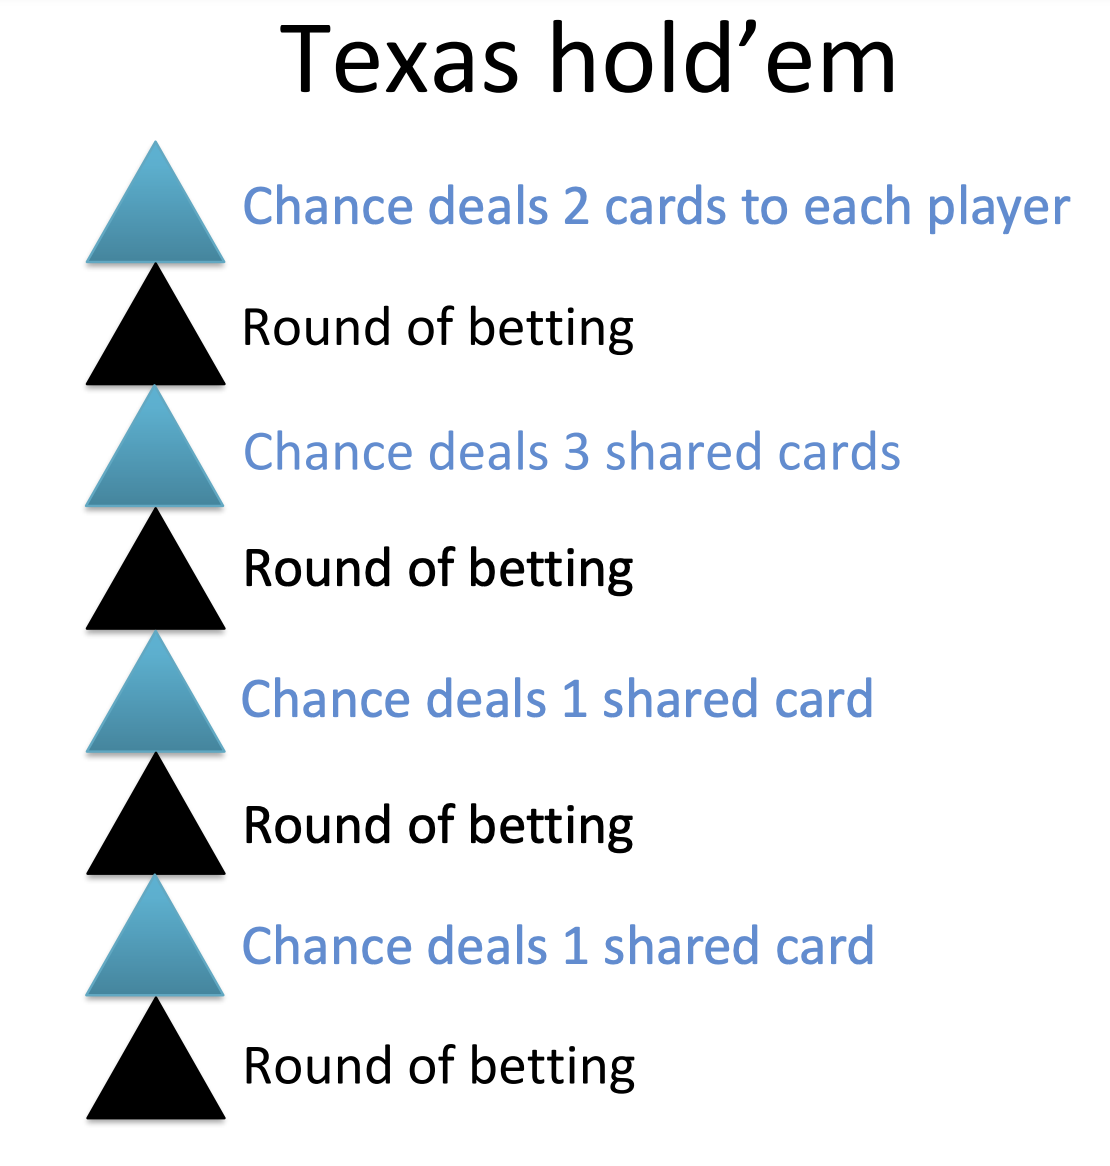
\includegraphics[width=7.5in,height=7.875in]{media/media/image1.png}

\href{https://www.youtube.com/watch?v=2dX0lwaQRX0}{\ul{https://www.youtube.com/watch?v=2dX0lwaQRX0}}

Sandholm's Research Paper

Sandholm's Research Paper

\href{https://www.science.org/doi/10.1126/science.aay2400}{\ul{https://www.science.org/doi/10.1126/science.aay2400}}

equilibrium concepts of von Neumann and Nash have been applied to many
real-world challenges such as auctions, cybersecurity, and pricing.

\begin{itemize}
\item
  The fundamental theorem of John von Neumann\textquotesingle s game
  theory states that in a broad category of games it is always possible
  to find an equilibrium from which neither player should deviate
  unilaterally
\item
  A Nash equilibrium is a list of strategies, one for each player, in
  which no player can improve by deviating to a different strategy.
  (class content, \#1 on homework)

  \begin{itemize}
  \item
    For example, the Nash equilibrium strategy for Rock-Paper-Scissors
    is to randomly pick Rock, Paper, or Scissors with equal probability.
    Against such a strategy, the best that an opponent can do in
    expectation is tie
  \item
    In this simple case, playing the Nash equilibrium also guarantees
    that the player will not win in expectation. However, in more
    complex games, even determining how to tie against a Nash
    equilibrium may be difficult; if the opponent ever chooses
    suboptimal actions, then playing the Nash equilibrium will indeed
    result in victory in expectation.
  \item
    In principle, playing the Nash equilibrium can be combined with
    opponent exploitation by initially playing the equilibrium strategy
    and then over time shifting to a strategy that exploits the
    opponent's observed weaknesses (for example, by switching to always
    playing Paper against an opponent that always plays Rock)
  \item
    Although a Nash equilibrium strategy is guaranteed to exist in any
    finite game, efficient algorithms for finding one are only proven to
    exist for special classes of games, among which two-player zero-sum
    games are the most prominent. No polynomial-time algorithm is known
    for finding a Nash equilibrium in two-player non-zero-sum games, and
    the existence of one would have sweeping surprising implications in
    computational complexity theory
  \end{itemize}
\item
  a stable state of a system involving the interaction of different
  participants, in which no participant can gain by a unilateral change
  of strategy if the strategies of the others remain unchanged.

  \begin{itemize}
  \item
    Personal note: Nash equilibrium in game theory is not the same as
    zugzwang in chess; while both involve a situation where a player is
    stuck with a strategy due to the actions of others, a Nash
    equilibrium implies a stable state where no player can improve their
    outcome by changing their strategy alone, whereas zugzwang means a
    player is forced to make a move that worsens their position because
    any move they make will be detrimental.
  \end{itemize}
\item
  Even if Nash is found:

  \begin{itemize}
  \item
    Moreover, even if a Nash equilibrium could be computed efficiently
    in a game with more than two players, it is not clear that playing
    such an equilibrium strategy would be wise. If each player in such a
    game independently computes and plays a Nash equilibrium, the list
    of strategies that they play (one strategy per player) may not be a
    Nash equilibrium and players might have an incentive to deviate to a
    different strategy.
  \end{itemize}
\end{itemize}


\includegraphics[width=7.5in,height=8.80556in]{media/media/image4.png}

\textbf{\ul{Pluribus:}}

\begin{itemize}
\item
  plays a fixed strategy that does not adapt to the observed tendencies
  of the opponents.
\item
  One example of this is the Lemonade Stand Game (17), illustrated in
  Fig. 1Opens in image viewer, in which each player simultaneously picks
  a point on a ring and wants to be as far away as possible from any
  other player.
\item
  The algorithms that we used to construct Pluribus, discussed in the
  next two sections, are not guaranteed to converge to a Nash
  equilibrium outside of two-player zero-sum games. Nevertheless, we
  observe that Pluribus plays a strong strategy in multiplayer poker
  that is capable of consistently defeating elite human professionals.
  This shows that even though the techniques do not have known strong
  theoretical guarantees on performance outside of the two-player
  zero-sum setting, they are nevertheless capable of producing
  superhuman strategies in a wider class of strategic settings
\item
  
\includegraphics[width=7.5in,height=3.625in]{media/media/image3.png}
\item
  HOW WAS THE STRATEGY MADE:

  \begin{itemize}
  \item
    The core of Pluribus's strategy was computed through self-play, in
    which the AI plays against copies of itself, without any data of
    human or prior AI play used as input. The AI starts from scratch by
    playing randomly and gradually improves as it determines which
    actions, and which probability distribution over those actions, lead
    to better outcomes against earlier versions of its strategy. Forms
    of self-play have previously been used to generate powerful AIs in
    two-player zero-sum games such as backgammon (18), Go (9, 19), Dota
    2 (20), StarCraft 2 (21), and two-player poker (4--6), though the
    precise algorithms that were used have varied widely. Although it is
    easy to construct toy games with more than two players in which
    commonly used self-play algorithms fail to converge to a meaningful
    solution (22), \textbf{\ul{in practice self-play has nevertheless
    been shown to do reasonably well in some games with more than two
    players}}
  \end{itemize}
\item
  \textbf{\ul{HOW IT WORKS:}}

  \begin{itemize}
  \item
    \textbf{\ul{(PHASE 1)}} Pluribus's self-play produces a strategy for
    the entire game offline, which we refer to as the blueprint
    strategy.

    \begin{itemize}
    \item
      Then during actual play against opponents, \textbf{\ul{(PHASE 2)}}
      Pluribus improves upon the blueprint strategy by searching for a
      better strategy in real time for the situations in which it finds
      itself during the game.
    \end{itemize}
  \end{itemize}
\item
  blueprint strategy in Pluribus was computed using a variant of
  counterfactual regret minimization (CFR)
\item
  CFR is an iterative self-play algorithm in which the AI starts by
  playing completely at random but gradually improves by learning to
  beat earlier versions of itself.

  \begin{itemize}
  \item
    Every competitive Texas hold'em AI for at least the past 6 years has
    computed its strategy using some variant of CFR
  \item
    We use a form of Monte Carlo CFR (MCCFR) that samples actions in the
    game tree rather than traversing the entire game tree on each
    iteration
  \end{itemize}
\item
  \textbf{\ul{Prices \& hardware allocations:}}

  \begin{itemize}
  \item
    The blueprint strategy for Pluribus was computed in 8 days on a
    64-core server for a total of 12,400 CPU core hours. It required
    less than 512 GB of memory. At current cloud computing spot instance
    rates, this would cost about \$144 to produce.
  \item
    This is in sharp contrast to all the other recent superhuman AI
    milestones for games, which used large numbers of servers and/or
    farms of graphics processing units (GPUs).
  \item
    More memory and computation would enable a finer-grained blueprint
    that would lead to better performance but would also result in
    Pluribus using more memory or being slower during real-time search.
  \item
    set the size of the blueprint strategy abstraction to allow Pluribus
    to run during live play on a machine with no more than 128 GB of
    memory while storing a compressed form of the blueprint strategy in
    memory.
  \end{itemize}
\item
  \textbf{Abstraction for large imperfect-information games}

  \begin{itemize}
  \item
    To reduce the complexity of the game, we eliminate some actions from
    consideration and also bucket similar decision points together in a
    process called abstraction (24, 25). After abstraction, the bucketed
    decision points are treated as identical. We use two kinds of
    abstraction in Pluribus: action abstraction and information
    abstraction.

    \begin{itemize}
    \item
      \textbf{\ul{Action abstraction:}}

      \begin{itemize}
      \item
        reduces the number of different actions the AI needs to
        consider.
      \item
        To reduce the complexity of forming a strategy, Pluribus only
        considers a few different bet sizes at any given decision point.
      \item
        The exact number of bets it considers varies between 1 and 14
        depending on the situation. Although Pluribus can limit itself
        to only betting one of a few different sizes between \$100 and
        \$10,000, when actually playing no-limit poker, \textbf{the
        opponents are not constrained to those few options.}
      \item
        What happens if an opponent bets \$150 while Pluribus has only
        been trained to consider bets of \$100 or \$200? Generally,
        Pluribus will rely on its search algorithm (described in a later
        section) to compute a response in real-time to such ``off-tree''
        actions.
      \end{itemize}
    \item
      \textbf{\ul{Information abstraction:}}

      \begin{itemize}
      \item
        decision points that are similar in terms of what information
        has been revealed (in poker, the player's cards and revealed
        board cards) are bucketed together and treated identically
      \item
        For example, a 10-high straight and a 9-high straight are
        distinct hands but are nevertheless strategically similar.
        Pluribus may bucket these hands together and treat them
        identically, thereby reducing the number of distinct situations
        for which it needs to determine a strategy.
      \item
        drastically reduces the complexity of the game, but it may wash
        away subtle differences that are important for superhuman
        performance.
      \item
        Therefore, during actual play against humans, Pluribus uses
        information abstraction only to reason about situations on
        future betting rounds, never the betting round that it is
        actually in. Information abstraction is also applied during
        offline self-play
      \end{itemize}
    \end{itemize}
  \end{itemize}
\item
  \href{https://aws.amazon.com/what-is/monte-carlo-simulation/}{\ul{Montecarlo
  simulation:}}

  \begin{itemize}
  \item
    a computational algorithm that uses random sampling to solve
    problems. It\textquotesingle s used to approximate functions and
    simulate the behavior of complex systems.
  \item
    The Monte Carlo simulation is a mathematical technique that predicts
    possible outcomes of an uncertain event.

    \begin{itemize}
    \item
      Computer programs use this method to analyze past data and predict
      a range of future outcomes based on a choice of action.
    \item
      For example, if you want to estimate the first month's sales of a
      new product, you can give the Monte Carlo simulation program your
      historical sales data.
    \item
      The program will estimate different sales values based on factors
      such as general market conditions, product price, and advertising
      budget.
    \end{itemize}
  \item
    The Monte Carlo simulation is a probabilistic model that can include
    an element of uncertainty or randomness in its prediction. When you
    use a probabilistic model to simulate an outcome, you will get
    different results each time. \textbf{For example, the distance
    between your home and office is fixed. However, a probabilistic
    simulation might predict different travel times by considering
    factors such as congestion, bad weather, and vehicle breakdowns.}
  \item
    In contrast, conventional forecasting methods are more
    deterministic. They provide a definite answer to the prediction and
    cannot factor in uncertainty. For instance, they might tell you the
    minimum and maximum travel time, but both answers are less accurate.
  \end{itemize}
\end{itemize}


\includegraphics[width=7.5in,height=6.91667in]{media/media/image2.png}

\textbf{Translating\,Pluribus‑style multi‑agent game‑solving to a
Mario\,Kart racing AI:}

Mario Kart is a multi-agent game.

\begin{longtable}[]{@{}
  >{\raggedright\arraybackslash}p{(\columnwidth - 4\tabcolsep) * \real{0.1980}}
  >{\raggedright\arraybackslash}p{(\columnwidth - 4\tabcolsep) * \real{0.4066}}
  >{\raggedright\arraybackslash}p{(\columnwidth - 4\tabcolsep) * \real{0.3954}}@{}}
\toprule\noalign{}
\begin{minipage}[b]{\linewidth}\raggedright
Poker ingredient
\end{minipage} & \begin{minipage}[b]{\linewidth}\raggedright
Mario\,Kart counterpart
\end{minipage} & \begin{minipage}[b]{\linewidth}\raggedright
Why it matters
\end{minipage} \\
\begin{minipage}[b]{\linewidth}\raggedright
Players (6\,elite pros)
\end{minipage} & \begin{minipage}[b]{\linewidth}\raggedright
Karts (8 racers, human or AI)
\end{minipage} & \begin{minipage}[b]{\linewidth}\raggedright
Non‑cooperative, each maximises finishing rank.
\end{minipage} \\
\begin{minipage}[b]{\linewidth}\raggedright
Hand + private cards
\end{minipage} & \begin{minipage}[b]{\linewidth}\raggedright
Current kart state (speed, drift angle, item inventory)
\end{minipage} & \begin{minipage}[b]{\linewidth}\raggedright
Imperfect information---opponents' item boxes are hidden.
\end{minipage} \\
\begin{minipage}[b]{\linewidth}\raggedright
Common cards / board
\end{minipage} & \begin{minipage}[b]{\linewidth}\raggedright
Track, item boxes, hazards
\end{minipage} & \begin{minipage}[b]{\linewidth}\raggedright
Shared but stochastic; items spawn randomly.
\end{minipage} \\
\begin{minipage}[b]{\linewidth}\raggedright
Bet sizes
\end{minipage} & \begin{minipage}[b]{\linewidth}\raggedright
Action primitives (steer left/right, accelerate, brake, drift, use item)
\end{minipage} & \begin{minipage}[b]{\linewidth}\raggedright
Requires action \emph{abstraction} to keep search tractable.
\end{minipage} \\
\begin{minipage}[b]{\linewidth}\raggedright
Pay‑off / chips
\end{minipage} & \begin{minipage}[b]{\linewidth}\raggedright
Lap time, rank, coins
\end{minipage} & \begin{minipage}[b]{\linewidth}\raggedright
Dense reward shaping possible (e.g. +time\,gain, --collision).
\end{minipage} \\
\midrule\noalign{}
\endhead
\bottomrule\noalign{}
\endlastfoot
\end{longtable}

\textbf{Thinking about a Blueprint\,+\,real‑time search → two‑level
racing brain}

\begin{longtable}[]{@{}
  >{\raggedright\arraybackslash}p{(\columnwidth - 4\tabcolsep) * \real{0.2059}}
  >{\raggedright\arraybackslash}p{(\columnwidth - 4\tabcolsep) * \real{0.3429}}
  >{\raggedright\arraybackslash}p{(\columnwidth - 4\tabcolsep) * \real{0.4512}}@{}}
\toprule\noalign{}
\begin{minipage}[b]{\linewidth}\raggedright
\textbf{Phase}
\end{minipage} & \begin{minipage}[b]{\linewidth}\raggedright
\textbf{Pluribus technique (poker)}
\end{minipage} & \begin{minipage}[b]{\linewidth}\raggedright
\textbf{Mario\,Kart adaptation}
\end{minipage} \\
\begin{minipage}[b]{\linewidth}\raggedright
\textbf{Offline self‑play to build a ``blueprint''}
\end{minipage} & \begin{minipage}[b]{\linewidth}\raggedright
Monte‑Carlo CFR over an \emph{abstracted} game tree\,
\end{minipage} & \begin{minipage}[b]{\linewidth}\raggedright
Train a \textbf{multi‑agent RL} policy (PPO/MADDPG) in the Mario\,Kart
simulator. Discretise the continuous controls into ≈\,10--20
macro‑actions (e.g. \emph{hard‑left‑drift + full‑throttle},
\emph{fire‑shell + hold‑line}).
\end{minipage} \\
\begin{minipage}[b]{\linewidth}\raggedright
\textbf{Runtime local improvement}
\end{minipage} & \begin{minipage}[b]{\linewidth}\raggedright
Depth‑limited search that re‑solves the subgame reached at each decision
point
\end{minipage} & \begin{minipage}[b]{\linewidth}\raggedright
Run a \textbf{model‑predictive game‑theoretic planner} each frame:

1. Sample opponents' next \emph{k} macro‑actions using their policy.

2. Solve a \textbf{dynamic game} for an approximate Nash equilibrium
trajectory (iterative best response)\,.

3. Execute the first control and repeat.
\end{minipage} \\
\midrule\noalign{}
\endhead
\bottomrule\noalign{}
\endlastfoot
\end{longtable}

\emph{Why split it?} The offline blueprint gives global race‑craft
(corner set‑ups, item economy) while the online solver reacts to
``banana‑split seconds'' like sudden shells or overtakes.

\textbf{Key engineering tricks (trying to mirror Pluribus)}

\begin{longtable}[]{@{}
  >{\raggedright\arraybackslash}p{(\columnwidth - 2\tabcolsep) * \real{0.2223}}
  >{\raggedright\arraybackslash}p{(\columnwidth - 2\tabcolsep) * \real{0.7777}}@{}}
\toprule\noalign{}
\begin{minipage}[b]{\linewidth}\raggedright
\textbf{Strategy Ideas}
\end{minipage} & \begin{minipage}[b]{\linewidth}\raggedright
\textbf{How to possibly use}
\end{minipage} \\
\begin{minipage}[b]{\linewidth}\raggedright
\textbf{Action abstraction}
\end{minipage} & \begin{minipage}[b]{\linewidth}\raggedright
Cluster wheel‑angle\,×\,throttle\,×\,drift combos into \textasciitilde N
``moves''. Items become extra discrete actions.
\end{minipage} \\
\begin{minipage}[b]{\linewidth}\raggedright
\textbf{Information abstraction}
\end{minipage} & \begin{minipage}[b]{\linewidth}\raggedright
Bucket track positions into sectors \& lane‑offset bins; bucket item
inventories into threat levels (``has red shell'', ``defence item'',
``empty'').
\end{minipage} \\
\begin{minipage}[b]{\linewidth}\raggedright
\textbf{Monte‑Carlo rollouts}
\end{minipage} & \begin{minipage}[b]{\linewidth}\raggedright
When an off‑tree event occurs (e.g. opponent uses Lightning you never
trained on), fall back to Monte‑Carlo sampling to estimate Q‑values for
novel states.
\end{minipage} \\
\begin{minipage}[b]{\linewidth}\raggedright
\textbf{Self‑play scalability}
\end{minipage} & \begin{minipage}[b]{\linewidth}\raggedright
Use domain‑randomised emulation (different tracks, karts, physics noise)
so the blueprint generalises---NeuralKart showed an emulator can run
fast enough for massive data\,.
\end{minipage} \\
\begin{minipage}[b]{\linewidth}\raggedright
\textbf{Computational budget}
\end{minipage} & \begin{minipage}[b]{\linewidth}\raggedright
Pluribus used ∼12\,k\,CPU‑hours\,; a similar budget buys
\textbf{hundreds of millions of simulated Kart frames}
\end{minipage} \\
\midrule\noalign{}
\endhead
\bottomrule\noalign{}
\endlastfoot
\end{longtable}

\href{https://cs231n.stanford.edu/reports/2017/pdfs/624.pdf}{\ul{https://cs231n.stanford.edu/reports/2017/pdfs/624.pdf}}

Can try:\\
Using offline self play MARL to learn a coarse ``blueprint'' policy,
then refine it in real time with a fast Nash‑equilibrium trajectory
solver that reasons about rivals' reactions---exactly the Pluribus
two‑phase recipe, but with karts instead of cards.

Tab 4

Tab 5

Translating Pluribus to Pokemon Gen 1 Random Battles

\begin{itemize}
\item
  Pluribus uses Iterative Monte Carlo CFR (MCCFR)

  \begin{itemize}
  \item
    variant of CFR that uses sampling to approximate the regret updates,
    making it more efficient for large game trees
  \end{itemize}
\item
  Similarities:

  \begin{itemize}
  \item
    They both have imperfect information
  \end{itemize}
\item
  Differences:

  \begin{itemize}
  \item
    Must adapt the algorithm to handle the sequential nature of Pokémon
    battles. In poker, everyone gets an individual independent move. In
    Pokemon, moves are sequential (both players make a choice, and
    that's it)
  \item
    Unlike poker, Pokemon battles have visible states, simplifying some
    aspects of decision-making.
  \end{itemize}
\item
  Must represent each game state as a node in the game tree.
\end{itemize}

Steps:

\begin{itemize}
\item
  Use random sampling to simulate different battle outcomes and then
  update regrets based on sampled outcomes.
\item
  Run multiple iterations
\item
  Although Libratus is meant to be played in 1v1 games
\end{itemize}

Tab 6

(base) mauriciogarcia@Mauricios-MacBook-Pro cfr\_web \% python
game\_loop.py

After 1000 games, win rate = 0.509

After 2000 games, win rate = 0.502

After 3000 games, win rate = 0.508

After 4000 games, win rate = 0.507

After 5000 games, win rate = 0.507

After 6000 games, win rate = 0.507

After 7000 games, win rate = 0.507

After 8000 games, win rate = 0.507

After 9000 games, win rate = 0.508

After 10000 games, win rate = 0.507

Final P1 win rate over 10000 games: 0.507

(base) mauriciogarcia@Mauricios-MacBook-Pro cfr\_web \%

\^{}Shows equilibrium was found

Tab 7

\end{document}
